\thispagestyle{fancy}
\vspace*{45pt}
\subsection{Tela comando impressoras}
 Esta tela é acessada pelo botão "IMP" ou "IMP X" sendo X o número da impressora atualmente selecionada de qualquer uma das telas de comando.
\begin{figure}[h]
  \centering
  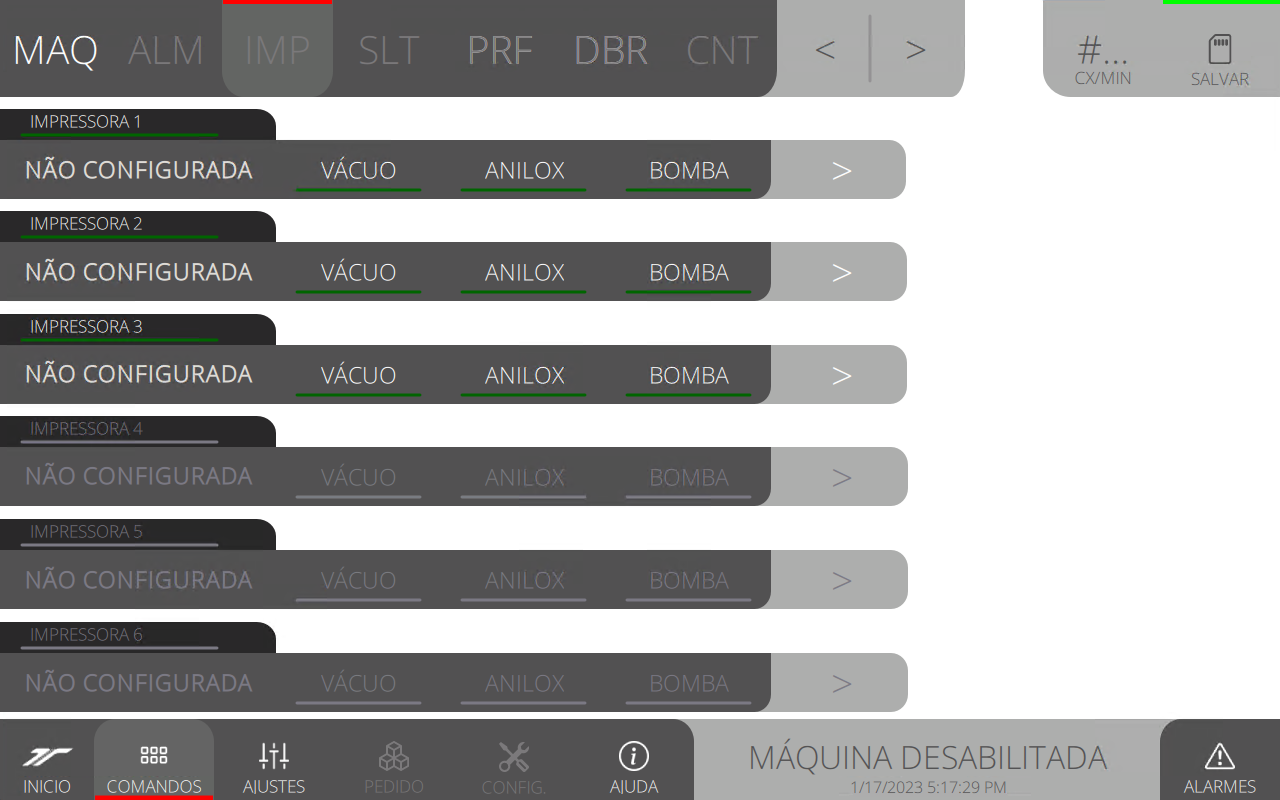
\includegraphics[width=576px,height=360px]{src/imagesFlexo/04-printter/01-printters/commands/e-Tela-Principal.png}
  \caption{ver depois.}
   \label{}
\end{figure}

\newpage
\thispagestyle{fancy}
\vspace*{\fill}
\subsubsection{\small{Visualização cor impressora}}
\begin{figure}[h]
  \centering
  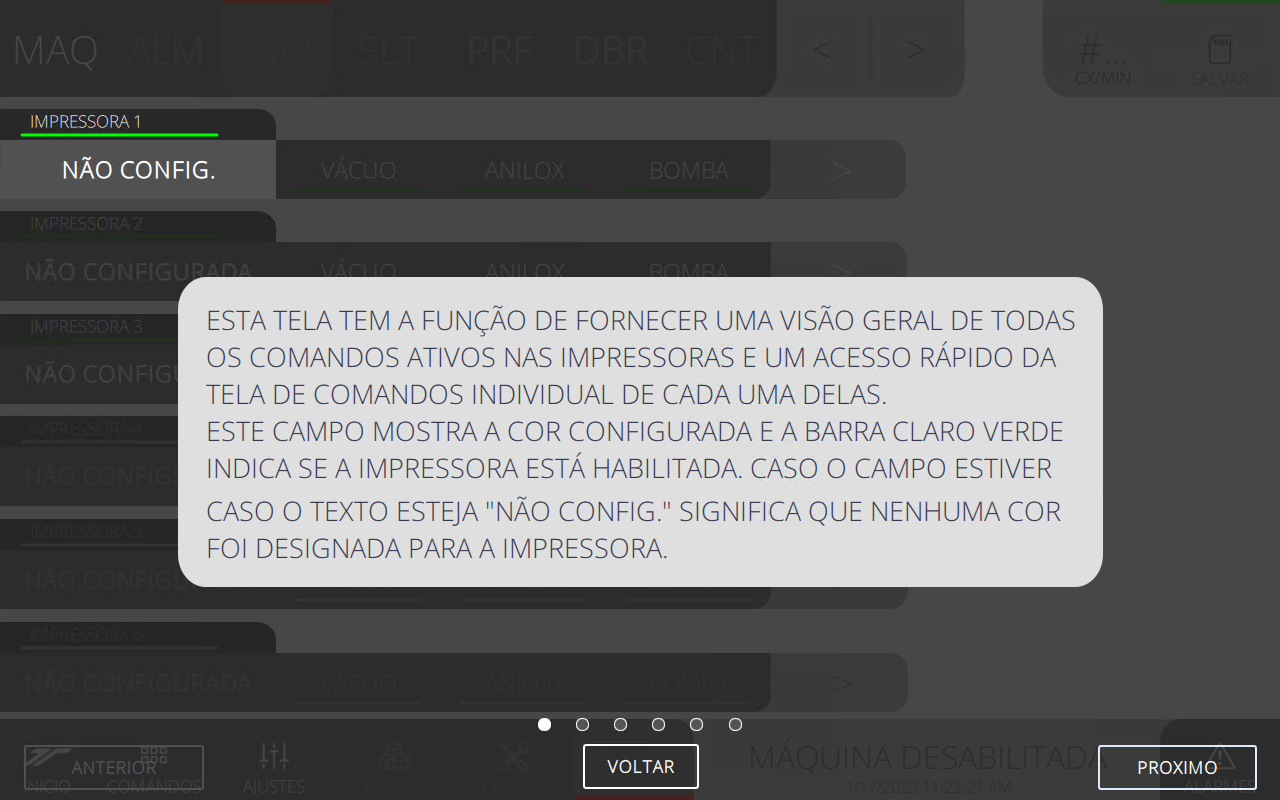
\includegraphics[width=576px,height=360px]{src/imagesFlexo/04-printter/01-printters/commands/e-1.png}
  \caption{ver depois.}
   \label{}
\end{figure}
\vspace*{\fill}

\newpage
\thispagestyle{fancy}
\vspace*{\fill}
\subsubsection{\small{Visualização se a aproximação do anilox está bloqueada}}
\begin{figure}[h]
  \centering
  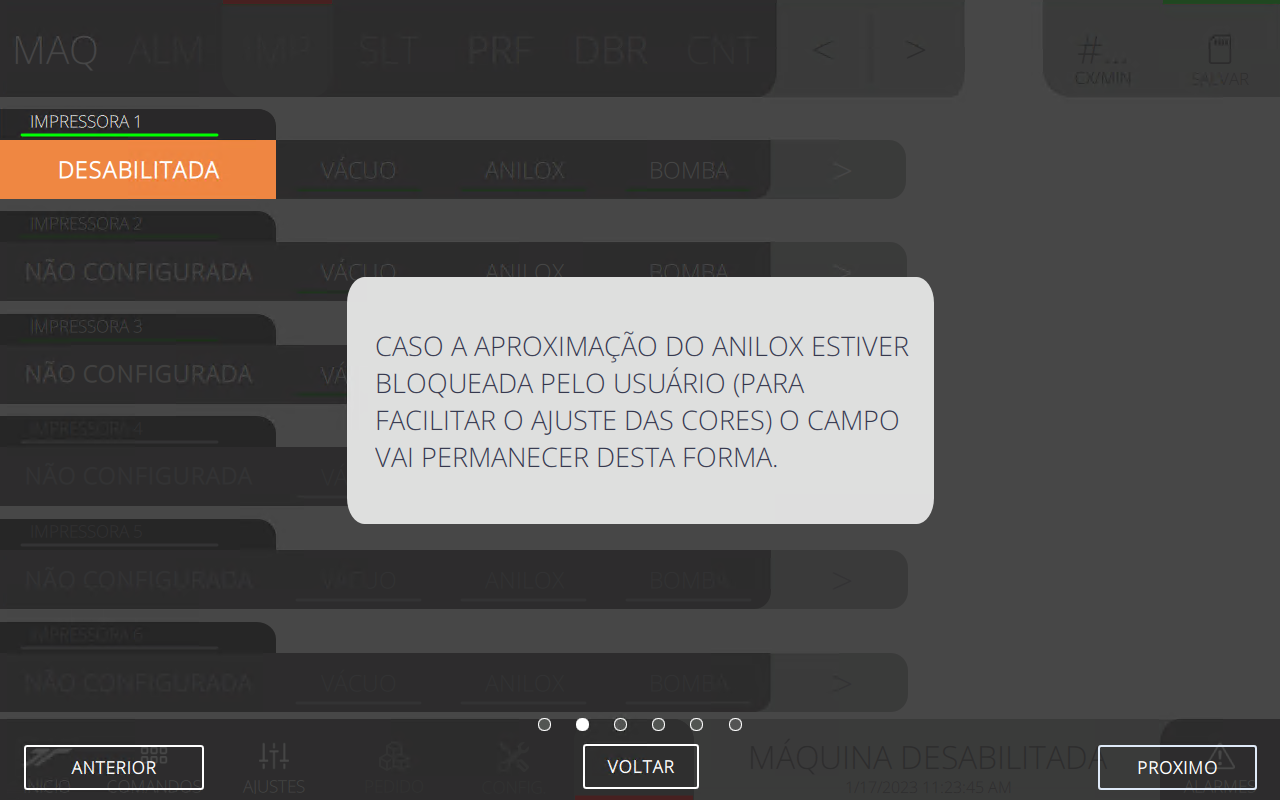
\includegraphics[width=576px,height=360px]{src/imagesFlexo/04-printter/01-printters/commands/e-2.png}
  \caption{ver depois.}
   \label{}
\end{figure}
\vspace*{\fill}

\newpage
\thispagestyle{fancy}
\vspace*{\fill}
\subsubsection{\small{Visualização vácuo habilitado}}
\begin{figure}[h]
  \centering
  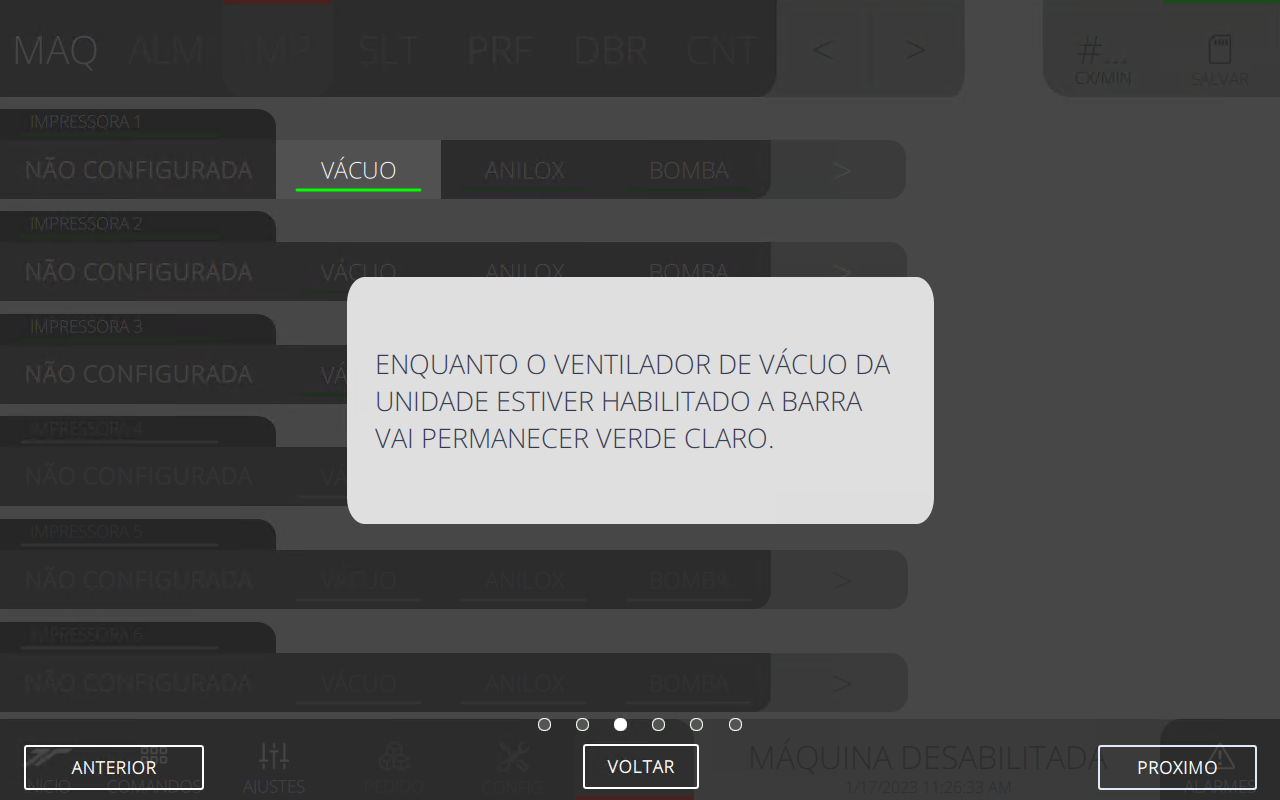
\includegraphics[width=576px,height=360px]{src/imagesFlexo/04-printter/01-printters/commands/e-3.png}
  \caption{ver depois.}
   \label{}
\end{figure}
\vspace*{\fill}

\newpage
\thispagestyle{fancy}
\vspace*{\fill}
\subsubsection{\small{Visualização giro anilox habilitado}}
\begin{figure}[h]
  \centering
  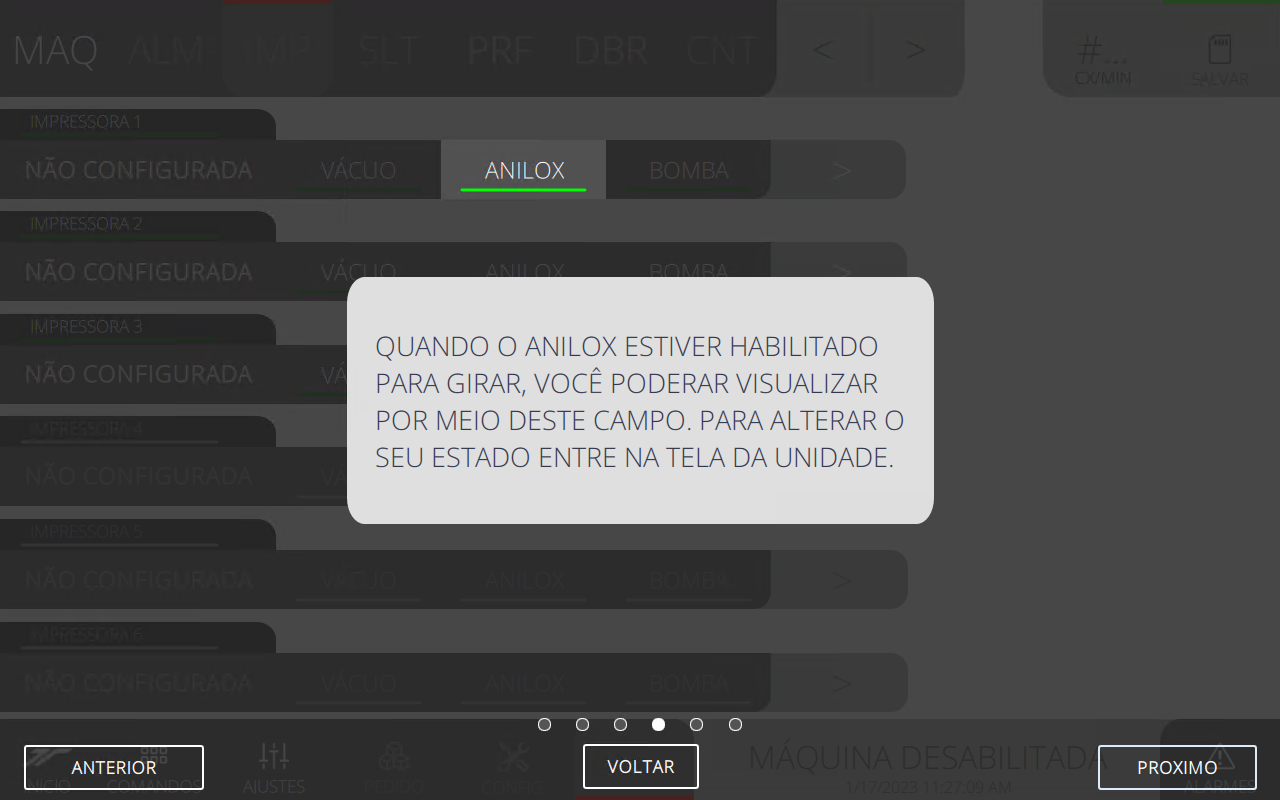
\includegraphics[width=576px,height=360px]{src/imagesFlexo/04-printter/01-printters/commands/e-4.png}
  \caption{ver depois.}
   \label{}
\end{figure}
\vspace*{\fill}

\newpage
\thispagestyle{fancy}
\vspace*{\fill}
\subsubsection{\small{Visualização lavagem de tinta habilitada}}
\begin{figure}[h]
  \centering
  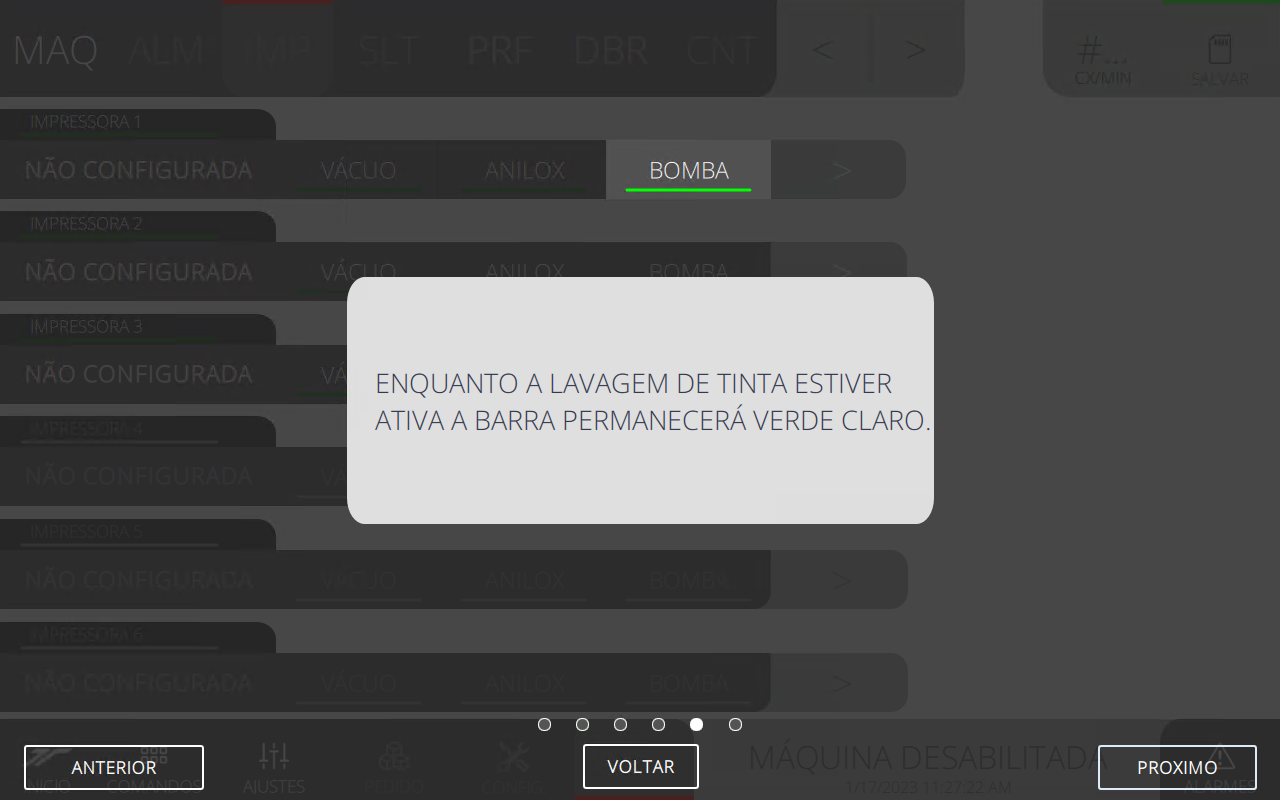
\includegraphics[width=576px,height=360px]{src/imagesFlexo/04-printter/01-printters/commands/e-5.png}
  \caption{ver depois.}
   \label{}
\end{figure}
\vspace*{\fill}

\newpage
\thispagestyle{fancy}
\vspace*{\fill}
\subsubsection{\small{Atalho para tela da impressora}}
\begin{figure}[h]
  \centering
  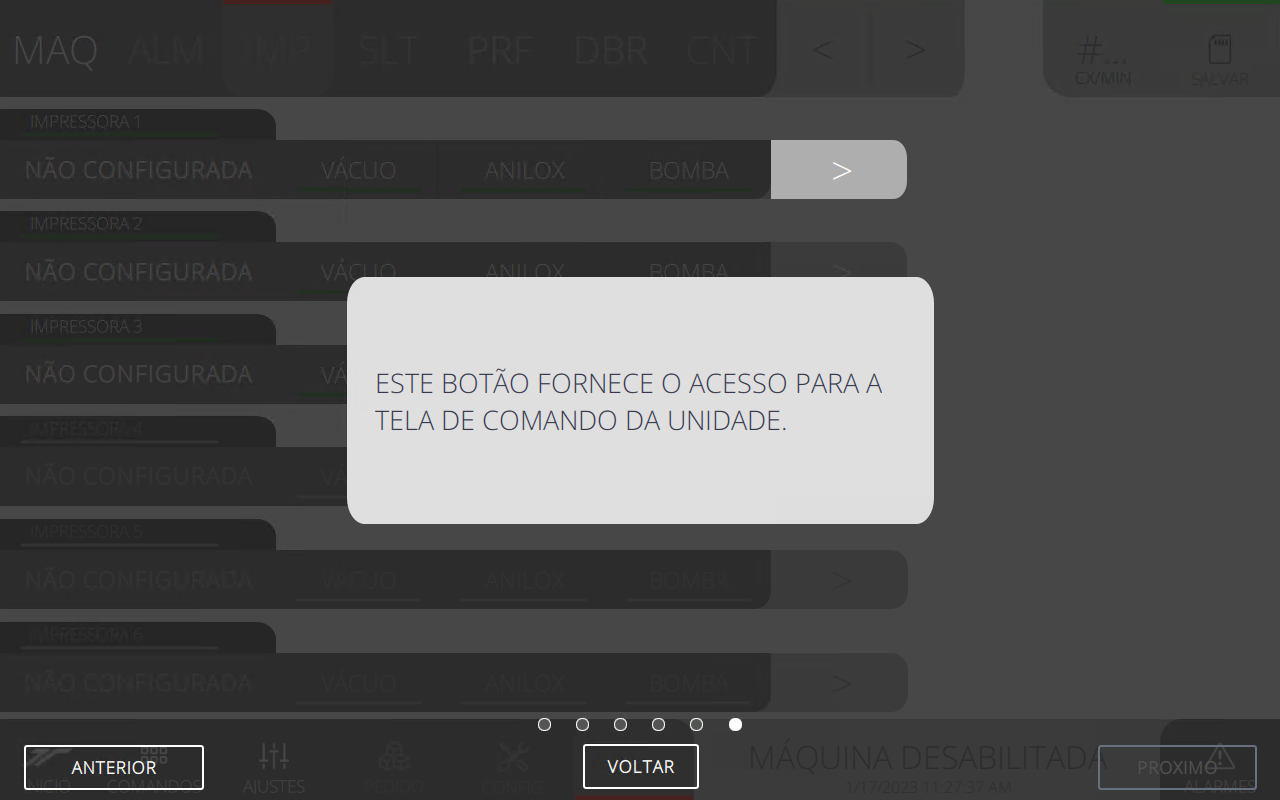
\includegraphics[width=576px,height=360px]{src/imagesFlexo/04-printter/01-printters/commands/e-6.png}
  \caption{ver depois.}
   \label{}
\end{figure}
\vspace*{\fill}

